% !TEX encoding = UTF-8 Unicode
\documentclass[a4paper]{article}

\usepackage{color}
\usepackage{url}
\usepackage[T2A]{fontenc} % enable Cyrillic fonts
\usepackage[utf8]{inputenc} % make weird characters work



\usepackage{graphicx}
\graphicspath{ {./slike/} }

\usepackage[english,serbian]{babel}
%\usepackage[english,serbianc]{babel} %ukljuciti babel sa ovim opcijama, umesto gornjim, ukoliko se koristi cirilica

\usepackage[unicode]{hyperref}
\hypersetup{colorlinks,citecolor=green,filecolor=green,linkcolor=blue,urlcolor=blue}

\usepackage{listings}

%\newtheorem{primer}{Пример}[section] %ćirilični primer
\newtheorem{primer}{Primer}[section]

\definecolor{mygreen}{rgb}{0,0.6,0}
\definecolor{mygray}{rgb}{0.5,0.5,0.5}
\definecolor{mymauve}{rgb}{0.58,0,0.82}

\lstset{ 
  backgroundcolor=\color{white},   % choose the background color; you must add \usepackage{color} or \usepackage{xcolor}; should come as last argument
  basicstyle=\scriptsize\ttfamily,        % the size of the fonts that are used for the code
  breakatwhitespace=false,         % sets if automatic breaks should only happen at whitespace
  breaklines=true,                 % sets automatic line breaking
  captionpos=b,                    % sets the caption-position to bottom
  commentstyle=\color{mygreen},    % comment style
  deletekeywords={...},            % if you want to delete keywords from the given language
  escapeinside={\%*}{*)},          % if you want to add LaTeX within your code
  extendedchars=true,              % lets you use non-ASCII characters; for 8-bits encodings only, does not work with UTF-8
  firstnumber=1000,                % start line enumeration with line 1000
  frame=single,	                   % adds a frame around the code
  keepspaces=true,                 % keeps spaces in text, useful for keeping indentation of code (possibly needs columns=flexible)
  keywordstyle=\color{blue},       % keyword style
  language=Python,                 % the language of the code
  morekeywords={*,...},            % if you want to add more keywords to the set
  numbers=left,                    % where to put the line-numbers; possible values are (none, left, right)
  numbersep=5pt,                   % how far the line-numbers are from the code
  numberstyle=\tiny\color{mygray}, % the style that is used for the line-numbers
  rulecolor=\color{black},         % if not set, the frame-color may be changed on line-breaks within not-black text (e.g. comments (green here))
  showspaces=false,                % show spaces everywhere adding particular underscores; it overrides 'showstringspaces'
  showstringspaces=false,          % underline spaces within strings only
  showtabs=false,                  % show tabs within strings adding particular underscores
  stepnumber=2,                    % the step between two line-numbers. If it's 1, each line will be numbered
  stringstyle=\color{mymauve},     % string literal style
  tabsize=2,	                   % sets default tabsize to 2 spaces
  title=\lstname                   % show the filename of files included with \lstinputlisting; also try caption instead of title
}




% Dodao Petar
\usepackage[]{algorithm2e}
\usepackage{subcaption}
%%%%%

\begin{document}

\title{Primene memetskog algoritma\\ \small{Seminarski rad u okviru kursa\\Metodologija stručnog i naučnog rada\\ Matematički fakultet}}

\author{Bogićević Marica, Karanović Boris, Košanin Petar, Šašić Filip\\ kontakt email prvog, drugog, trećeg, četvrtog autora}

%\date{9.~april 2015.}

\maketitle

\abstract{
TODO}

\tableofcontents

\newpage

\section{Uvod}
\label{sec:uvod}

TODO



\section{Primene memetskog algoritma}
\label{sec:primene_memetskog_algoritma}
TODO


\subsection{Problem bojenja grafa}
\label{sec:bojenje_grafa}
Neka je zadat graf $G = (V, E)$, gde je $V$ skup čvorova, a $E$ skup grana tog grafa. Bojenje grafa $G$ predstavlja problem dodeljivanja ''boja'' elementima grafa\footnote{Problem isključivo zavisi od \textit{broja} boja, a ne od konkretnih boja.}. Bojenje čvorova je pridruživanje po jedne boje svakom čvoru grafa $G$. Dodavanjem ograničenja maksimalnog broja boja, dobijamo problem k-bojenja grafa. \textit{Ispravno k-bojenje grafa} $G$ je ono za koje ne postoje dva susedna čvora\footnote{Dva čvora su susedna, ako postoji grana koja ih povezuje.} koji su obojeni istom bojom. Drugim rečima, ispravno k-bojenje grafa deli čvorove skupa $V$ u $k$ nezavisnih podskupova, pri čemu jedan taj podskup čine nesusedni čvorovi, obojeni istom bojom.


\begin{figure}[h!]
	\centering

	\begin{subfigure}[normla]{0.3\textwidth}
		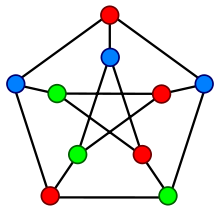
\includegraphics[scale=0.3]{bojene_grafa1}
		\caption{Primer ispravnog bojenja čvorova grafa}
		\label{bojenje_grafa1}
	\end{subfigure}
	~
	\begin{subfigure}[normla]{0.3\textwidth}
		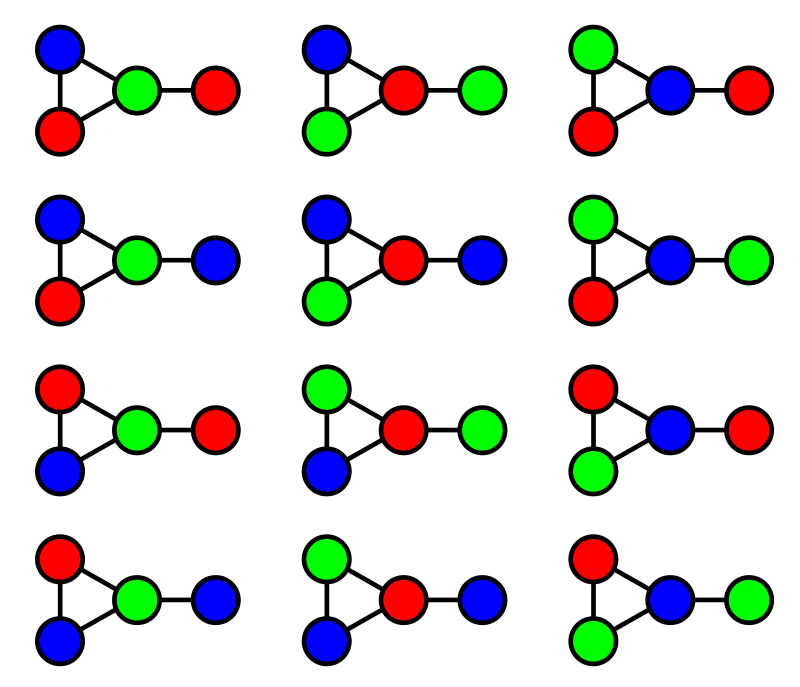
\includegraphics[scale=0.1]{bojenje_grafa2}
		\caption{Različita ispravna bojenja čvorova grafa}
		\label{bojenje_grafa2}
	\end{subfigure}
		\caption{Slika (a) prikazuje ispravno 3-bojenje Pitersonovog grafa, dok na slici (b) prikazano je 12 različitih načina 3-bojanja grafa. Izvor slika \cite{graph_coloring} }
\label{bojene_grafa}
\end{figure}

TODO



\subsection{Problem trgovačkog putnika}
\label{sec:trgovacki_putnik}

TODO
















\subsection{Problem prepoznavanja zajednica}
\label{sec:prepoznavanje_zajednica}

TODO












\section{Zaključak}
\label{sec:zakljucak}

TODO

\addcontentsline{toc}{section}{Literatura}
\appendix
\bibliography{seminarski} 
\bibliographystyle{plain}

\appendix
\section{Dodatak}
TODO


\end{document}
